\id{МРНТИ 81.93.29}{}

\begin{articleheader}
\sectionwithauthors{M.M. Yesmagambetova, A.S. Amirova, I.Yu. Petrova, T.U. Yesmagambetov, T.L. Ten}{SIMULATION AND MITIGATION OF DATA POISONING ATTACKS IN MACHINE LEARNING}

{\bfseries
\textsuperscript{1}M.M. Yesmagambetova\alink{https://orcid.org/0000-0001-9273-7402},
\textsuperscript{2}A.S. Amirova\alink{https://orcid.org/0000-0002-5715-4954}\textsuperscript{\envelope },
\textsuperscript{3}I.Yu. Petrova\alink{https://orcid.org/0000-0001-7231-5368},
\textsuperscript{1}T.U. Yesmagambetov\alink{https://orcid.org/0009-0000-3268-867X},
\textsuperscript{1}T.L. Ten\alink{https://orcid.org/0000-0002-9677-0266}
}
\end{articleheader}

\begin{affiliation}
\textsuperscript{1}Karaganda University of Kazpotrebsouz, Karaganda, Kazakhstan,

\textsuperscript{2}Astana IT University, Astana, Kazakhstan,

\textsuperscript{3}Astrakhan State Technical University, Astrakhan, Russia

\raggedright \textsuperscript{\envelope }Corresponding author: akzhibek.amirova@astanait.edu.kz
\end{affiliation}

Machine learning (ML) models are increasingly used in mission-critical
applications and are therefore vulnerable to adversarial attacks. Data
poisoning attack is one such threat, in which an adversary injects
specially designed samples into training data, which can cause a sudden
drop in model accuracy or even intentionally bias its decisions in favor
of the attacker. This paper presents a simulation of a data poisoning
attack on machine learning using MATLAB. Experimental results show that
data poisoning can significantly reduce classification accuracy, but
using data cleaning techniques can restore model performance. A
mitigation method is also proposed that combines the ideas of ensemble
learning, outlier prediction estimation, and marginal outlier filtering.
Although the main components of the method are widely known, their
combination to combat data poisoning attacks is original. Data
visualization, decision boundary construction, and accuracy analysis
confirm the effectiveness of the mitigation measures. The proposed
approach can be useful for developers of secure machine learning systems
and researchers studying the resilience of models to adversarial
influences. Future research may focus on developing more advanced
defense mechanisms such as trust-based learning methods or adaptive
attack detection algorithms.

{\bfseries Keywords:} machine learning (ML), data poisoning attacks,
availability attack, ensemble learning, out-of-bag (OOB) prediction.

\begin{articleheader}
{\bfseries МАШИНАЛЫҚ ОҚЫТУДАҒЫ ДЕРЕКТЕРДІ БҰЗУ ШАБУЫЛДАРЫН МОДЕЛЬДЕУ ЖӘНЕ ОНЫ ЖЕҢІЛДЕТУ}

{\bfseries
\textsuperscript{1}М.М. Есмагамбетова,
\textsuperscript{2}А.С. Амирова\textsuperscript{\envelope },
\textsuperscript{3}И.Ю. Петрова,
\textsuperscript{1}Т.У. Есмагамбетов,
\textsuperscript{1}Т.Л. Тен
}
\end{articleheader}

\begin{affiliation}
\textsuperscript{1}Қазтұтынуодағы Қарағанды университеті, Қарағанды, Қазақстан,

\textsuperscript{2}Astana IT University, Астана, Қазақстан,

\textsuperscript{3}Астрахань мемлекеттік техникалық университеті, Астрахань, Ресей

e-mail:akzhibek.amirova@astanait.edu.kz
\end{affiliation}

Машиналық оқыту (ML) үлгілері миссия үшін маңызды қолданбаларда көбірек
пайдаланылады және сондықтан қарсыластық шабуылдарына осал. Деректерді
улану шабуылы - шабуылдаушы жаттығу деректеріне арнайы әзірленген
үлгілерді енгізетін осындай қауіптердің бірі, бұл модель дәлдігінің
кенеттен төмендеуіне әкелуі мүмкін немесе тіпті оның шешімдерін
шабуылдаушы пайдасына әдейі бұрмалауы мүмкін. Бұл мақалада MATLAB
көмегімен машиналық оқытудағы деректерді улану шабуылының симуляциясы
ұсынылған. Эксперименттік нәтижелер деректерді улану жіктеу дәлдігін
айтарлықтай төмендетуі мүмкін екенін көрсетеді, бірақ деректерді тазалау
әдістерін пайдалану үлгі өнімділігін қалпына келтіре алады. Сондай-ақ
ансамбльдік оқыту, бағалау, жоспарланбаған қателерді болжау және шекті
шектен шығуларды сүзгілеу идеяларын біріктіретін шабуылдың осы түрін
жұмсарту әдісі ұсынылды. Әдістің негізгі құрамдас бөліктері кеңінен
белгілі болғанымен, деректердің улану шабуылдарымен күресу үшін олардың
комбинациясы түпнұсқа болып табылады. Деректерді визуализациялау, шешім
шекарасын құру және дәлдік талдауы қорғау шараларының тиімділігін
растайды. Ұсынылған тәсіл қауіпсіз машиналық оқыту жүйелерін
әзірлеушілер мен модельдердің дұшпандық әсерлерге төзімділігін
зерттейтін зерттеушілер үшін пайдалы болуы мүмкін. Болашақ зерттеулер
сенімге негізделген оқыту әдістері немесе бейімді шабуылдарды анықтау
алгоритмдері сияқты жетілдірілген қорғаныс механизмдерін әзірлеуге
бағытталуы мүмкін.

{\bfseries Түйін сөздер:} машиналық оқыту (ML), деректерді бұзу шабуылдары,
қолжетімділік шабуылдары, ансамбльді оқыту, жоспарланбаған қателерді
болжау.

\begin{articleheader}
{\bfseries МОДЕЛИРОВАНИЕ И СМЯГЧЕНИЕ АТАК ОТРАВЛЕНИЯ ДАННЫХ В МАШИННОМ ОБУЧЕНИИ}

{\bfseries
\textsuperscript{1}М.М.Есмагамбетова,
\textsuperscript{2}А.С.Амирова\textsuperscript{\envelope },
\textsuperscript{3}И.Ю.Петрова,
\textsuperscript{1}Т.У.Есмагамбетов,
\textsuperscript{1}Т.Л.Тен
}
\end{articleheader}

\begin{affiliation}
\textsuperscript{1}Карагандинский университет Казпотребсоюза, Караганда, Казахстан,

\textsuperscript{2}Astana IT University, Астана, Казахстан,

\textsuperscript{3}Астраханский государственный технический университет, Астрахань, Россия

e-mail: akzhibek.amirova@astanait.edu.kz
\end{affiliation}

Модели машинного обучения (ML) все чаще используются в критически важных
приложениях и, следовательно, уязвимы для состязательных атак. Атака
отравления данных - одна из таких угроз, при которой злоумышленник
внедряет специально разработанные образцы в обучающие данные, что может
привести к внезапному падению точности модели или даже намеренно
исказить ее решения в пользу злоумышленника. В статье приведено
моделирование атаки отравления данных на машинное обучение с
использованием MATLAB. Экспериментальные результаты показывают, что
отравление данных может значительно снизить точность классификации, но
использование методов очистки данных позволяет восстановить
производительность модели. Также был предложен метод смягчения данного
вида атак, объединяющий идеи ансамблевого обучения, оценки
прогнозирование внеплановой ошибки и фильтрации маргинальных выбросов.
Хотя основные компоненты метода широко известны, их комбинация для
борьбы с атаками отравления данных является оригинальной. Визуализация
данных, построение границы принятия решений и анализ точности
подтверждают эффективность мер защиты. Предложенный подход может быть
полезен для разработчиков безопасных систем машинного обучения и
исследователей, изучающих устойчивость моделей к враждебным
воздействиям. Будущие исследования могут быть сосредоточены на
разработке более продвинутых механизмов защиты, таких как методы
обучения на основе доверия или адаптивные алгоритмы обнаружения атак.

{\bfseries Ключевые слова:} машинное обучение (ML), атаки с искажением
данных, атаки на доступность, ансамблевое обучение, прогнозирование
внеплановой ошибки.

\begin{multicols}{2}
{\bfseries Introduction.} Modern machine learning models are widely used in
various fields, including medical diagnostics, autonomous systems,
cybersecurity, and the financial sector {[}1{]}. However, their
vulnerability to attacks aimed at disrupting the correctness of their
operation remains one of the key problems in the field of artificial
intelligence. One of the most dangerous types of adversarial influences
is a data poisoning attack, in which an attacker deliberately modifies
the training data set in order to degrade the quality of the
model' s predictions or impose predetermined decisions on
it {[}2{]}.

The relevance of the study is determined by the growing number of real
attacks on machine learning systems and the increase in their potential
damage. In recent years, the problem of model resilience to attacks has
attracted significant attention from the scientific community. The works
{[}3, 4{]} showed that even small changes in the data can significantly
reduce the accuracy of classification. Despite this, effective
mechanisms for protecting against data poisoning are still under active
study.

The purpose of the work is to develop and analyze a method of protection
against data poisoning attacks based on outlier processing and anomaly
filtering.

To achieve this goal, the following tasks are solved:

-simulate a data poisoning attack and evaluate its impact on the
accuracy of the model;

- research various methods for detecting abnormal data and propose a
method of protection;

- implement an experimental verification of the protection method in
MATLAB;

- evaluate the effectiveness of the proposed method based on the
accuracy metrics of the model before and after protection.

The hypothesis of the study is that the use of data cleaning methods at
the preprocessing stage can significantly increase the resilience of
machine learning models to data poisoning attacks, while maintaining
their accuracy and generalization ability.

The theoretical significance of the study lies in expanding knowledge
about the impact of data poisoning attacks on machine learning and
possible protection mechanisms. The practical significance of the work
is due to the applicability of the proposed method in real ML systems
exposed to external threats.

Thus, the presented study is aimed at studying and developing effective
ways to counter one of the most serious threats to machine learning
security.

{\bfseries Materials and methods.} A data poisoning attack is an attack on
machine learning algorithms in which an attacker intentionally
introduces malicious data into the training set in order to degrade the
accuracy of the model or cause it to make incorrect decisions {[}5{]}.

In recent years, data poisoning attacks have become one of the most
discussed issues in the field of machine learning security. The main
goal of such attacks is to intentionally introduce malicious examples
into the training dataset in order to degrade the quality of the model
or change its behavior on test data {[}6{]}.

One of the earliest and most frequently cited efforts in this regard is
the work of Biggio et al. {[}7{]}, in which the authors demonstrated
that it is possible to reduce the accuracy of support vector machine
models significantly even if a small percentage of poisoned data is
added to the training set. In the paper, there is considerable
description of various attack scenarios as well as initial suggestions
regarding how the vulnerability of training algorithms can be analyzed.

More recent research, e.g., the research by Munoz-Gonzalez et al.
{[}8{]}, has generalized the idea of data poisoning attacks by utilizing
inverse gradient optimization techniques to develop poisoned examples
that are capable of attacking contemporary deep neural networks. These
works have demonstrated that attacks can not only be directed towards
lowering the overall accuracy, but also at modifying the behavior of the
model in some situations.

On the other hand, considerable attention has been paid to the
development of mitigation methods for data poisoning attacks. One
approach is to develop robust learning algorithms that can reduce the
impact of poisoned data. For example, Steinhardt et al. {[}9{]} proposed
a certified protection method that provides guarantees of model
robustness in the presence of a limited amount of attack data.

Other studies focus on pre-cleaning training data from anomalous
examples. Classical outlier detection methods such as Isolation Forest
{[}10{]} and Local Outlier Factor (LOF) {[}11{]} are widely used to
identify anomalies. However, as work shows, simply removing outliers may
not be sufficient, since attack data is often crafted to look similar to
normal data.

Types of Data Poisoning Attacks in Machine Learning

In machine learning, data poisoning attacks are a serious threat that
involve deliberately changing the data used to train a model in order to
degrade its performance or introduce certain vulnerabilities. There are
several key types of this class of attacks, differing in their goals and
methods of implementation.

One of the common types is an availability attack. The main goal of this
attack is to significantly reduce the accuracy of the model on all input
data, which makes it unsuitable for practical use. To implement such an
attack, attackers can introduce random noise into the training dataset
or change class labels in an arbitrary order, which leads to incorrect
training of the model and its subsequent inoperability {[}12{]}.

Another type is an attack on the target behavior, during which the
attacker seeks to achieve a systematic error in the model when
processing specific input data. Unlike an availability attack, here the
data corruption is targeted and affects mainly certain classes or
instances. This can be used, for example, to make a machine learning
model misclassify images of a certain object or misinterpret specific
signals {[}13{]}.

Another dangerous technique is a backdoor attack, the main goal of which
is to introduce a hidden mechanism (trigger) into the model. During
standard operation, the model behaves correctly, but when a certain
input signal or pattern appears, it begins to make deliberate errors.
This can be done, for example, by adding images with imperceptible but
specific changes to the training set, which can be used in the future by
attackers to activate the embedded vulnerability {[}14{]}.

The above-discussed forms of data poisoning attacks illustrate various
methods of jeopardizing a machine learning model from general loss in
accuracy to strategically injecting covert flaws. Estimating the effect
of such attacks and designing defense approaches involves an intensive
investigation that spans multiple stages. The following is the procedure
of carrying out an experiment for modeling attacks, building a model,
and subsequently probing the efficacy of defense strategies.

The evaluation of the impact of a data poisoning attack on a machine
learning model follows a sequence of steps (Figure 1).
\end{multicols}

\begin{figure}[H]
	\centering
	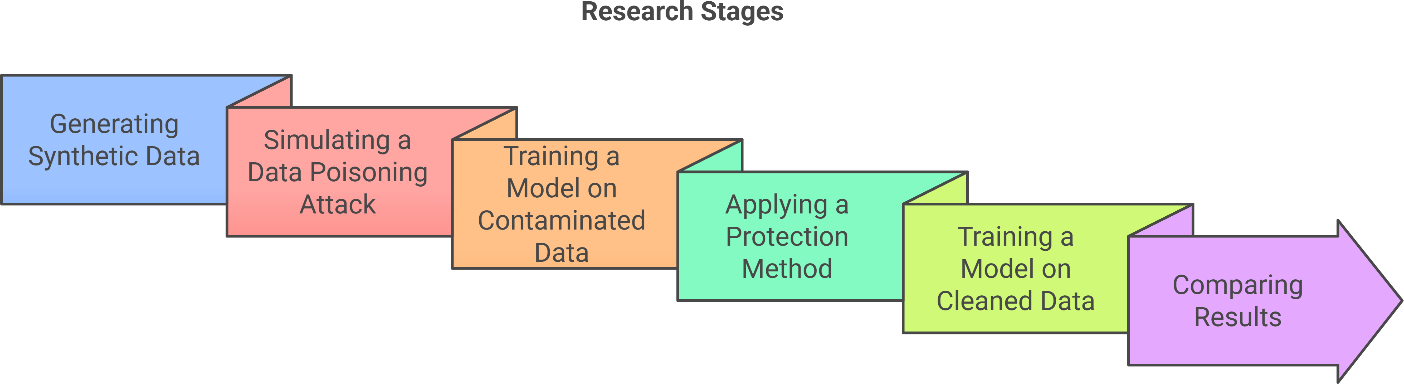
\includegraphics[width=0.8\textwidth]{media/ict2/image224}
	\caption*{Fig.1 - The data poisoning attack impact evaluation algorithm}
\end{figure}

\begin{multicols}{2}
The first step is generating synthetic data, whereby you can replicate a
controlled environment for study. Data used can be artificially
generated samples simulating real-world cases, which helps in
replicating data poisoning scenarios and their subsequent analysis.

The second step is simulating a data poisoning attack. In this step, the
source data is intentionally compromised, such as altering class labels,
adding noise instances, or adding hidden patterns that can affect the
process of model training. Based on the objective of the study,
availability attacks, targeted attacks, or backdoor attacks can be used.

The third stage involves training a model on contaminated data. During
the training process, the model is trained on a corrupted data set,
which allows us to assess the impact of the attack on its accuracy and
overall performance.

Finally, a protection method is deployed to eradicate the impact of the
attack. This could be through some data cleaning mechanisms, robust
learning, or utilizing other anomaly detection algorithms.

Then, after applying a protection method, the model is retrained on
cleaned data, which corresponds to the task of training a model on
cleaned data. This allows us to test how effective the proposed
protection method is and understand up to which point we are able to
regain the original accuracy of the model.

The final step is one of comparison of results. The comparison of the
accuracy of the model trained on infected data and the model trained
after the implementation of the protection method enables us to evaluate
the effectiveness of the suggested approach quantitatively. Primary
attention is drawn to the alteration of classification accuracy, the
degree of resistance of the model to attacks, and its capacity to
preserve generalizing properties after being exposed to malicious data.

To mitigate data poisoning attacks, a method is proposed that combines
the ideas of ensemble learning, out-of-bag prediction evaluation, and
margin filtering of outliers.

The training dataset is first contaminated with poisoned examples, which
leads to a decrease in the accuracy of the model. To eliminate the
impact of such anomalous data, an approach is used based on the analysis
of the model confidence through out-of-bag (OOB) predictions of an
ensemble classifier trained using the bagging method.

1. Training the ensemble classifier.

An ensemble classifier is trained on the poisoned dataset with the
labels Xpoisoned and Ypoisoned. During the training process, OOB
predictions are calculated for each training example, which allows us to
estimate the "confidence" of the model without the need for additional
validation.

2. Calculating the margin.

In the binary classification task, we employ an ensemble of 𝑀 base
classifiers built using the bootstrap bagging method. For each object 𝑥𝑖
in the training set, there is a subset of classifiers that did not see
that object during training (the so-called Out-Of-Bag, or OOB,
classifiers). Let \(\mathcal{J}_{OOB}(x_{i})\) denote the set of indices
of these OOB classifiers and let
\(M_{OOB}\left( x_{i} \right) = \left| \mathcal{J}_{OOB}(x_{i}) \right|\)
be their number.

Each classifier \(h_{j}\) produces a binary prediction
\(h_{j}(x_{i}) \in \left\{ + 1, - 1 \right\}\). For convenience, we
define the following scores for the probabilities of belonging to class
+1 and class −1 based on the OOB predictions:

\[score_{i}^{(1)} = \frac{1}{M_{OOB}(x_{i})}\sum_{j \in \mathcal{J}_{OOB}(x_{i})}^{}{I\left( h_{j}\left( x_{i} \right) = + 1 \right)\ ,}\]

\[score_{i}^{(2)} = 1 - score_{i}^{(1)}\ ,\]

where \(I( \cdot )\) is an indicator function that equals 1
if the condition inside the parentheses is met, and 0 otherwise. Thus,
\(score_{i}^{(1)}\) represents the fraction of OOB classifiers that
voted for class +1, while \(score_{i}^{(2)}\) is the fraction that voted
for class −1. After obtaining these OOB-based scores for each object
\(x_{i}\), we compute the ``margin,'' which is a measure of the
ensemble's confidence in its prediction. One common way to define the
margin \(score_{i}^{(2)}\)in binary classification is to take the
absolute difference between \(score_{i}^{(1)}\) and \(score_{i}^{(2)}\):

\[margin_{i} = \left| score_{i}^{(1)} - score_{i}^{(2)} \right| = \left| 2score_{i}^{(1)} - 1 \right|\]

The value \(margin_{i}\) reflects the ensemble's level of ``confidence''

If \(margin_{i}\) is close to 1, most OOB classifiers have voted for the
same class, indicating a ``reliable'' prediction.

If \(margin_{i} \approx 0\), it means the votes from OOB classifiers are
almost evenly split, and the ensemble is uncertain about the object's
class. This scenario may signify an anomaly or be the result of
``poisoned'' data.

3. Identifying and removing outliers.

Based on the distribution of margin values, a threshold is determined,
for example, equal to the 20th percentile. Examples with a margin below
this threshold are interpreted as anomalous and excluded from the
training set. Thus, the remaining subset of data is considered more
reliable for further training.

4. Retraining the classifier.

On the cleaned dataset, the main model is retrained, which helps to
mitigate the negative impact of poisoning and improve the final
classification accuracy.

The Matlab software environment was used to simulate the data poisoning
attack.

{\bfseries Results and Discussion.} Figure 2 shows part of a script for
simulating a data poisoning attack, in particular an attack on
availability.

Figure 3 shows three graphs describing the original, clean data on which
the model is trained, and the data after the data poisoning attack has
been implemented. The first graph clearly shows the division between the
two classes: the red crosses (×) represent class -1 points, and the blue
circles (o) represent class 1 points. The distribution of the points
shows that the data is well separated, as there is a noticeable gap
between the two groups. This allows the model to build a clear decision
boundary, which contributes to high accuracy when classifying new
examples. The second graph shows that poisoned points located closer to
the boundary between the classes were added to the original set, making
them less distinguishable. In addition, some of the class labels were
flipped, meaning that objects from one class were labeled as belonging
to another. This blurs the boundary between the classes and creates
areas where the model may get confused when classifying. As a result,
its ability to correctly recognize new data is reduced, which is the
goal of the attack.
\end{multicols}

\begin{figure}[H]
	\centering
	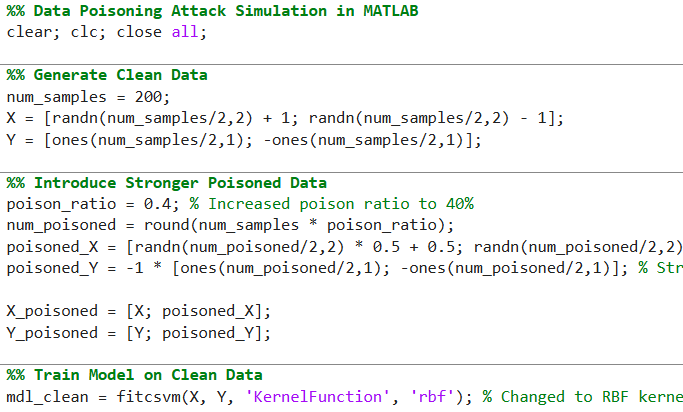
\includegraphics[width=0.8\textwidth]{media/ict2/image225}
	\caption*{Fig.2 - Matlab script}
\end{figure}

\begin{multicols}{2}
The following results were obtained: accuracy on clean model: 94.00\%,
accuracy on poisoned model: 83.00\%, accuracy on mitigated model:
87.00\%.

There are a number of important points to note in the comparison of this
method with existing approaches. In the first place, powerful learning
methods such as robust SVM with loss correction or weighted training
samples attempt to reduce the sensitivity of the model to outlier data
by minimizing it during optimization. They do so by requesting
modifications to be introduced into the learning method, which may prove
difficult to implement and be transferred across varied architectures.
Conversely, the new method works on the level of pre-cleaning the data,
enabling us to disentangle the step of removing anomalies from the step
of training the main model and include it in standard machine learning
pipelines.

Second, there exist some outlier detection techniques like Isolation
Forest and Local Outlier Factor (LOF), which are oriented to detecting
anomalous samples. However, they do typically require fine-tuning of
hyperparameters and sensitivity to data, especially in cases where
attack data is crafted to simulate normal example distributions. With
our approach, using the OOB predictions of the ensemble classifier for
computing the margin allows for a natural estimate of uncertainty that
facilitates more effective normal vs. abnormal discrimination without
additional tuning burdens.

Third, some modern methods recommend iterative data cleansing methods,
such as leave-one-out testing of the impact of individual instances on
model performance or inverse gradient optimization methods. Although
these can be very accurate, they are computationally intensive and
require sophisticated setting up, limiting their realistic application
in real-time. The advantage of OOB Margin Filtering is that it is a
single pass through the data with OOB predictions, which has
significantly less computational expense.
\end{multicols}

\begin{figure}[H]
    \centering
    \begin{subfigure}[t]{0.45\textwidth}
        \centering
        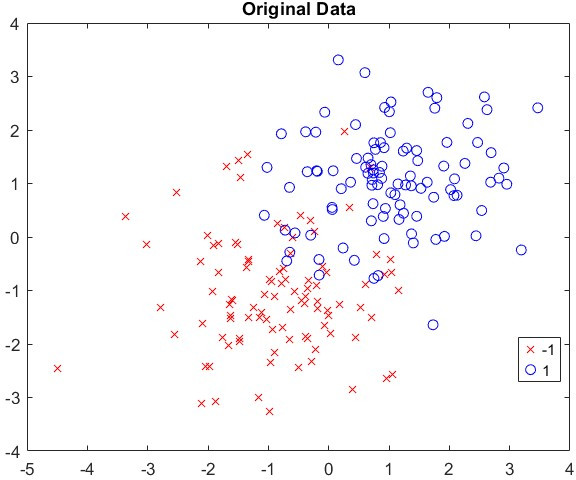
\includegraphics[width=\textwidth]{media/ict2/image226}
    \end{subfigure}
    \begin{subfigure}[t]{0.45\textwidth}
        \centering
        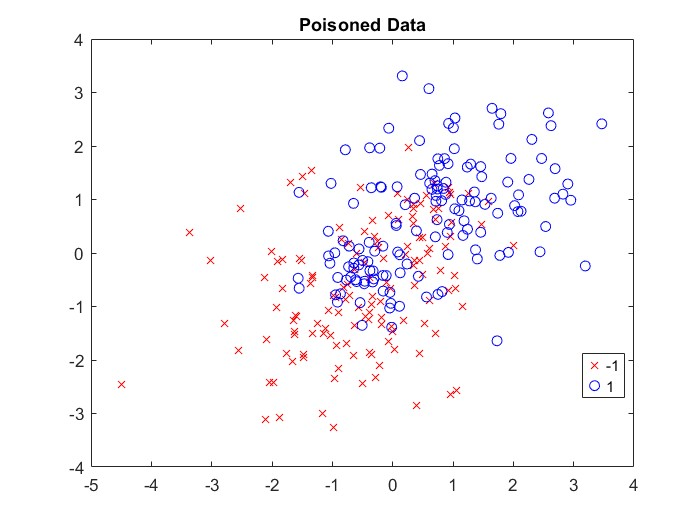
\includegraphics[width=\textwidth]{media/ict2/image227}
    \end{subfigure}
    \begin{subfigure}[t]{0.45\textwidth}
        \centering
        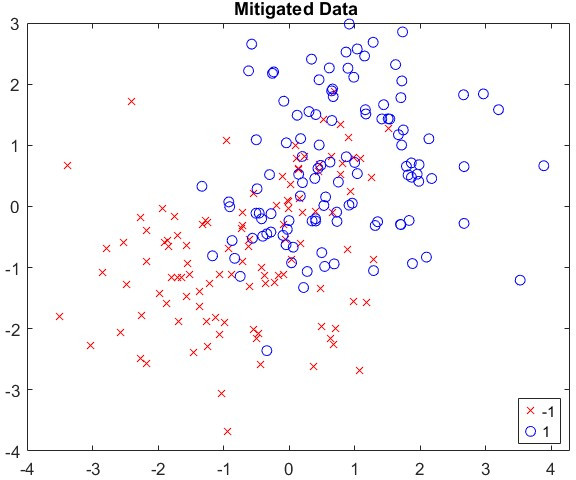
\includegraphics[width=\textwidth]{media/ict2/image228}
    \end{subfigure}
    \caption*{{\bfseries Fig.3 - Graphs for original, poisoned and mitigated data}}
\end{figure}

\begin{multicols}{2}
Finally, in terms of originality, the method described here has
individual well-researched components (OOB prediction analysis, margin
calculation, and outlier filtering), but their combination to combat
data poisoning attacks is a new idea that doesn' t have a
proven title in the literature. Compared to the certified protection
methods, our approach is simpler and more flexible, and hence it is
possible to apply it in situations of limited computational resources
and for many models. Thus, the proposed method is an efficient,
computation-light, and easy-to-implement solution for pre-cleaning
training data with poisoned samples. Its usefulness is validated by
experimental run suggesting higher model accuracy when performed with a
purified dataset, and in comparison with existing approaches, there is
hope for real application in the area of data poisoning attacks.

{\bfseries Conclusion.} The proposed method combines the ideas of ensemble
learning, out-of-bag prediction estimation, and marginal outlier
filtering. Although the basic components of the method are widely known,
their combination for combating data poisoning attacks is original.
Experimental results show that the application of this method can
significantly improve the accuracy of the model compared to the model
trained on contaminated data, and also demonstrates computational
efficiency and ease of implementation, which allows integrating it into
existing machine learning pipelines without significant costs. Further
comparison with existing methods can be carried out in empirical
studies, where the effectiveness of filtering and subsequent training of
the model will be assessed.
\end{multicols}

\begin{center}
{\bfseries References}
\end{center}

\begin{references}
1. Nithya T. et al. A comprehensive survey of machine learning:
Advancements, applications, and challenges //2023 Second International
Conference on Augmented Intelligence and Sustainable Systems (ICAISS). -
IEEE, 2023. - P.354-361. DOI
\href{http://dx.doi.org/10.1109/ICAISS58487.2023.10250547}{10.1109/ICAISS58487.2023.10250547}

2. Sun G. et al. Data poisoning attacks on federated machine learning
//IEEE Internet of Things Journal. - 2021. - Т.9(13). - P.11365-11375.
DOI
\href{http://dx.doi.org/10.1109/JIOT.2021.3128646}{10.1109/JIOT.2021.3128646}

3. Muñoz-González L. et al. Towards poisoning of deep learning algorithms
with back-gradient optimization //Proceedings of the 10th ACM workshop
on artificial intelligence and security. -- 2017. - P.27-38. DOI
\href{http://dx.doi.org/10.48550/arXiv.1708.08689}{10.48550/arXiv.1708.08689}

4. Koh P. W., Steinhardt J., Liang P. Stronger data poisoning attacks
break data sanitization defenses //Machine Learning. - 2022. - P.1-47.
DOI 10.48550/arXiv.1811.00741

5. Tolpegin V. et al. Data poisoning attacks against federated learning
systems //Computer security -- ESORICs 2020: 25th European symposium on
research in computer security, ESORICs 2020, guildford, UK, September
14-18, 2020, proceedings, part i 25. - Springer International
Publishing, 2020. - P.480-501. DOI 10.48550/arXiv.2007.08432

6. Cinà A. E. et al. Machine learning security against data poisoning:
Are we there yet? //Computer. - 2024. -Т.57(3). - С.26-34. DOI
10.1109/MC.2023.3299572

7. Biggio B., Nelson B., Laskov P. Poisoning attacks against support
vector machines //arXiv preprint arXiv:1206.6389. - 2012. DOI
10.48550/arXiv.1206.6389

8. Muñoz-González L. et al. Towards poisoning of deep learning algorithms
with back-gradient optimization //Proceedings of the 10th ACM workshop
on artificial intelligence and security. -- 2017. - P.27-38. DOI
\href{http://dx.doi.org/10.48550/arXiv.1708.08689}{10.48550/arXiv.1708.08689}

9. Steinhardt J., Koh P. W. W., Liang P. S. Certified defenses for data
poisoning attacks //Advances in neural information processing systems. -
2017. DOI 10.48550/arXiv.1706.03691

10. Liu F. T., Ting K. M., Zhou Z. H. Isolation forest //2008 eighth ieee
international conference on data mining. -- IEEE, 2008. -- P.413-422.
DOI \href{http://dx.doi.org/10.1109/ICDM.2008.17}{10.1109/ICDM.2008.17}

Breunig M. M. et al. LOF: identifying density-based local outliers
//Proceedings of the 2000 ACM SIGMOD international conference on
Management of data.- 2000.-Vol.29(2)- P.93-104.
\href{https://doi.org/10.1145/335191.335388}{DOI 10.1145/335191.33538}

11. Miao C. et al. Towards data poisoning attacks in crowd sensing
systems //Proceedings of the Eighteenth ACM International Symposium on
Mobile Ad Hoc Networking and Computing. -- 2018. - P.111-120. DOI
10.1145/3209582.3209594

12. Fan J. et al. A survey on data poisoning attacks and defenses //2022
7th IEEE International Conference on Data Science in Cyberspace (DSC).
-- IEEE, 2022. -- P.48-55. DOI
\href{http://dx.doi.org/10.1109/DSC55868.2022.00014}{10.1109/DSC55868.2022.00014}

13. Schwarzschild A. et al. Just how toxic is data poisoning? a unified
benchmark for backdoor and data poisoning attacks //International
Conference on Machine Learning. -- PMLR, 2021. -- P.9389-9398. DOI
10.48550/arXiv.2006.12557
\end{references}

\begin{authorinfo}
\emph{{\bfseries Information about the authors}}

Amirova A.S. - PhD, assistant professor, Astana IT University, Astana,
Kazakhstan, e-mail: akzhibek.amirova@astanait.edu.kz;

Yesmagambetova M.M.- PhD, assistant professor, Karaganda University of
Kazpotrebsoyuz, Karaganda, Kazakhstan e-mail: marzhan1983@mail.ru;

Yesmagambetov T.U.- master, senior lecturer, Karaganda University of
Kazpotrebsoyuz, Karaganda, Kazakhstan e-mail: \\Timur198300@mail.ru;

Petrova I.Yu. - Doctor of Technical Sciences, Professor, Department of
Higher and Applied Mathematics, Astrakhan State Technical University,
e-mail irina.petrova1011@gmail.com;

Ten T.L. - Doctor of Technical Sciences, Professor, Karaganda University
of Kazpotrebsoyuz, Karaganda, Kazakhstan e-mail: Tentl@mail.ru/

\emph{{\bfseries Сведения об авторах}}

Амирова А.С. - PhD, ассистент профессор, Astana IT University, Астана,
Казахстан, e-mail: \\akzhibek.amirova@astanait.edu.kz;

Есмагамбетова М.М. - PhD, доцент - Карагандинский университет
Казпотребсоюза, Караганда, Казахстан e-mail: \\marzhan1983@mail.ru;

Есмагамбетов Т.У.- магистр, старший преподаватель - Карагандинский
университет Казпотребсоюза, Караганда, Казахстан e-mail: Timur198300@mail.ru;

Петрова И.Ю. - доктор технических наук, профессор, кафедра Высшая и
прикладная математика Астраханского государственного
технического университета, e-mail irina.petrova1011@gmail.com;

Тен Т.Л. - доктор технических наук, профессор, Карагандинский
университет Казпотребсоюза, Караганда, Казахстан e-mail: Tentl@mail.ru
\end{authorinfo}
